%Autor: Simon Walker
%Version: 1.0
%Datum: 10.11.2019

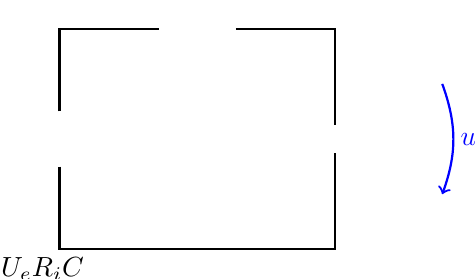
\begin{tikzpicture}[thick,scale=0.7, every node/.style={scale=0.7}]%[xscale=0.6, yscale=0.6]
	
	%\draw[help lines] (0,0) grid (9, 5);
	\normalsize
	
	% Spannungsquelle
	\tzUV{0.5}{2.5}{$U_e$}{r}{+}
	
	% Leitungen
	%Ue - Ri
	\draw (0.5, 3) -- (0.5, 4.5) -- (2.3, 4.5);
	%Ri - C
	\draw (3.7, 4.5) -- (5.5, 4.5) -- (5.5, 2.75);
	%C - Ue
	\draw (0.5, 2) -- (0.5, 0.5) -- (5.5, 0.5) -- (5.5, 2.25); 
	
	% Widerstand R1
	\tzRH{3}{4.5}{$R_i$}{b}
		
	% Kondensator C (mitte 7.5, 2.5)
	\tzCV{5.5}{2.5}{$C$}{l}
	
	% Spannungspfeil über Kondensator
	\draw [->,thick ,blue] (6.5, 3.5) to [out=-70, in=70] (6.5, 1.5); 
	\node [blue, right] at (6.7, 2.5) {\Large $u_C(t)$};
	
	
\end{tikzpicture}
